
\documentclass{article}
\usepackage{graphicx}
\usepackage{dot2texi}
\makeatletter
\@ifundefined{verbatim@out}{\newwrite\verbatim@out}{}
\makeatother
\usepackage{tikz}
\usetikzlibrary{shapes,arrows}
% \usepackage[pdf]{graphviz}
%\usepackage{feynmp}
\usepackage{subfigure}
\graphicspath{{figs/}}

\title{Deep Learning Notes}

\author{Peter Thompson}

\begin{document}

% TODO:
% add stuff on notation, make sure we get this right
% add more to stuff on matrix dimensions and indices
% add more on gradient saturation/relu/leaky relu
% Forward propagation
% BackPropagation
% Cost function - start from logistic loss - generalise to cross entropy

\section{random notes}
Don't use sigmoid as an activation function. Tanh is generally superior, as it has a mean of zero (sigmoid has a mean of 0.5). Nonzero mean can make training more difficult in subsequent layers. Tanh has a mean of zero. May want a sigmoid as a final activation function (that is, in the output layer) when doing a binary classification problem.

relu is generally good.

\begin{figure}
% \begin{dot2tex}
% digraph G {
%     node [shape="circle"];
%     a_1 -> a_2 -> a_3 -> a_4 -> a_1;
%   }
% \end{dot2tex}
\begin{dot2tex}[mathmode]
digraph network1 {
rankdir=LR;
node [shape=circle];
subgraph inputlayer {
    node [shape=none];
    x_1 [label="x_1^2"];
    x_2 [label="x_2^2"];
    label="input layer";
    };
{x_1 x_2} -> {a_1 a_2 a_3 a_4} -> {o_1};
}
\end{dot2tex}
\caption{a network}
\end{figure}


% \begin{dot2tex}[mathmode]
% digraph network1 {
% rankdir=LR;
% subgraph inputlayer {
%     node [shape=none];
%     x1, x2 ;
%     label="input layer";
%     };
% {x1 x2} -> {a_1 a_2 a_3 a_4} -> {o_1};
% }
% \end{dot2tex}
% \caption{a network}
% \end{figure}

% subgraph inputlayer {
%     node [shape=none];
%     x1, x22 ;
%     label="input layer";
% };
% subgraph hiddenlayer{
%     node [shape=square];
%     a_1, a_2, a_3, a_4;
%     label="hidden layer";
% };
% subgraph outputlayer{
%     node [shape=circle];
%     o_1;
%     label="output layer";
% };
% {x_1 x_2} -> {a_1 a_2 a_3 a_4} -> {o_1};


\section{Notation}

\subsection{Matrix Dimensions/network layout/notation}
A network consists of $L$ layers. The $l$th layer contains $n_l$ neurons, or nodes. Each layer of the network consists of a number of neurons. Each layer of neurons applies an activation function to a vector of inputs $Z^l$ to produce a vector of outouts, or activations $A^l$, such that
\begin{eqnarray*}
A^l &=& f(Z^l) \\
& =& f(W^lA^{l-1} + b^l)
\end{eqnarray*}
Where $W^l$ is a matrix of weights for layer $l$ and $b^l$ is a vector of biases. The weight vector acts on the prior layer of activations, or the first layer acts on the raw inputs. for $m$ training examples, the raw inputs $X$ (or $A^0$) has dimensions $(n^0,m)$, and each the weight matrix for each layer has dimension $(n^l,n^{l-1})$. 

square brackets in the superscript denote the layer. Round brackets in the superscript denote the training example (column for X,Y), squiggly brackets denote the mini batch number used in batched gradient descent.
Note that training epoch refers to the numer of traversals through the training dataset.




% A couple quick notes:
% \begin{itemize}
%     \item Each {\bf column} of the input, $X$, corresponds to an observation/example of the features. 
%     \item The weight matrix for layer $l$ should have dimensions $(n^l,n^{l-1})$, where $n^l$ is the number of nodes in layer $l$. The initial inputs, $X$, can be thought of as the activations of layer $l=0$. 
% \end{itemize}

\section{Loss and Cost functions}

Loss function is the loss/error associated with a single training example
Cost function is the loss computed over all examples

\subsection{logistic loss}

Think of $\hat{y}$ as the conditional probability $\hat{y}(x) = P(y=1|x)$. Based on our model, the probability $y=0$ is then $P(y=0|x) = 1 - \hat{y}$. For a single observation, these two outcomes can be summarised as
\begin{equation}
P(y|x) = \hat{y}^y(1-\hat{y})^{(1-y)}
\end{equation}
For a set of $(y_i,x_i)$ observations, $(Y,X)$, the likelihood of a given model is given by the product of the conditional probabilities
\begin{eqnarray*}
L(W|X) & = & P(Y|X) \\
& = & \prod_i P(y_i|x_i) \\
& = & \prod_i \hat{y}_i^{y_i}(1-\hat{y}_i)^{(1-y_i)}
\end{eqnarray*}
where $\hat{y}$ is described by our model, and is a function of $W$ and $x$.
% The above is for a single example. The likelihood (of parameters) for a given training set would be obtained from the product $\prod_i P(y_i|x_i)$, where $\hat(y)_i$ is a function of $x_i$.

The cost function from logistic loss can then be obtained from the negative log likelihood of $L(W|X)$ above
\begin{eqnarray*}
J(W,x) & = & - \log L(W|X) \\
 & = & \sum_i  (y_i-1) \log(1 - \hat{y}_i) - y_i \log(\hat{y}_i)
\end{eqnarray*}
The log of the product reduces to a sum over logs.

The cross entropy is a measure of dissimilarity between two different distributions, $p$ and $q$. 
\begin{equation}
H(p,q) = \sum_i p_i \log q_i
\end{equation}
The sum here runs over the values that $y$ can take (0 or 1), i.e. the dependant variable of the distributions $p$ and $q$. 

If we interpret $p$ as the distribution of $y$ and $q$ as the distribution of $\hat{y}$, then for our binary classification case we have $y \in \{0,1\}$, $p \in \{1-y,y\}$ and $q \in \{1-\hat{y},\hat{y}\}$.
The cross entropy for a single example is then
\begin{eqnarray*}
H(p,q) & = & - \sum_i p_i \log(q_i) \\
 & = & - \left( (1-y) \log (1-\hat{y}) + y \log \hat{y}\right)
\end{eqnarray*}
The cost function obtained by averaging $H(p,q)$ over all samples is then
\begin{eqnarray*}
J(W|X) & = & \frac{1}{N}\sum_n^N H(p_n,q_n) \\
 & = &  \frac{-1}{N} \left((1-y_n) \log (1-\hat{y}_n) + y \log \hat{y}_n\right)
\end{eqnarray*}
Which is equivalent (up to a constant factor) to the cost function obtained from logistic loss above. Minimising cross entropy in this case is equivalent to minimising the logistic loss, which results in the maximum likelihood estimate for the parameters $W$ of the model $\hat{y}$.


\section{activation functions and their derivatives}


\subsection{sigmoid}
Sigmoid used to be the default activation function, but in recent times ReLu has proven to be more popular/perform better. Sigmoid is still good for an output function (i.e. activation function in the output layer) in binary classification tasks.
The sigmoid function (or logit function) and its derivative are given by
\begin{eqnarray*}
\sigma(x) & = &\frac{1}{1 - e^{-x}} \\
\frac{d\sigma(x)}{dx} & = & \sigma(x)(1 - \sigma(x)) \\
\end{eqnarray*}

these are plotted below
\begin{figure}[tb]
\begin{centering}
\subfigure{
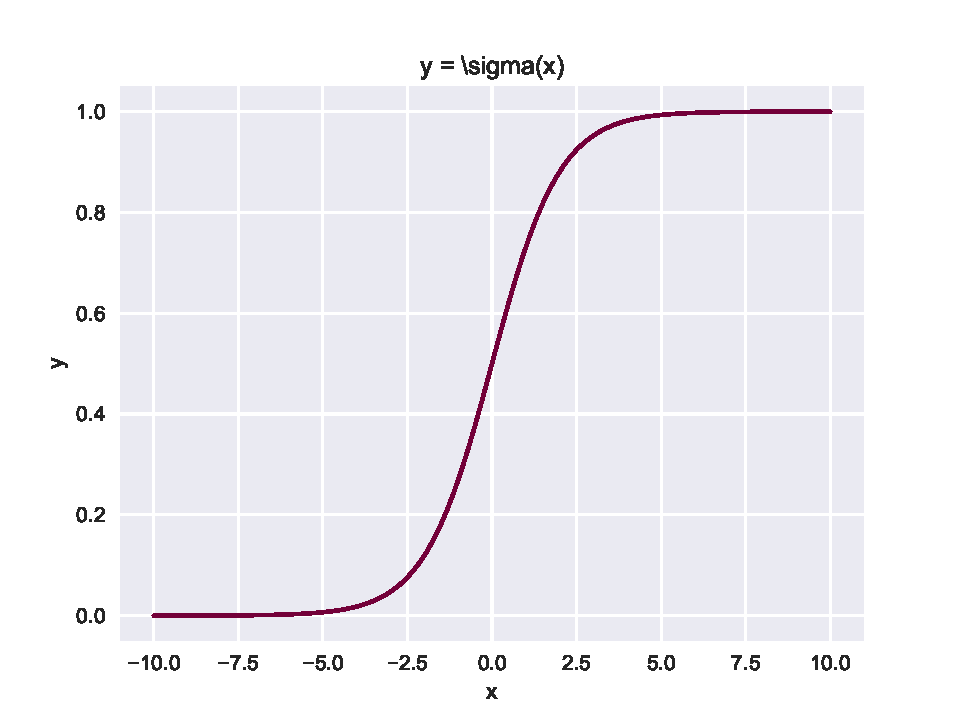
\includegraphics[width=0.45\linewidth,angle=0]{sigmoid.pdf}
% \caption{sigmoid activation function}
}
\subfigure{
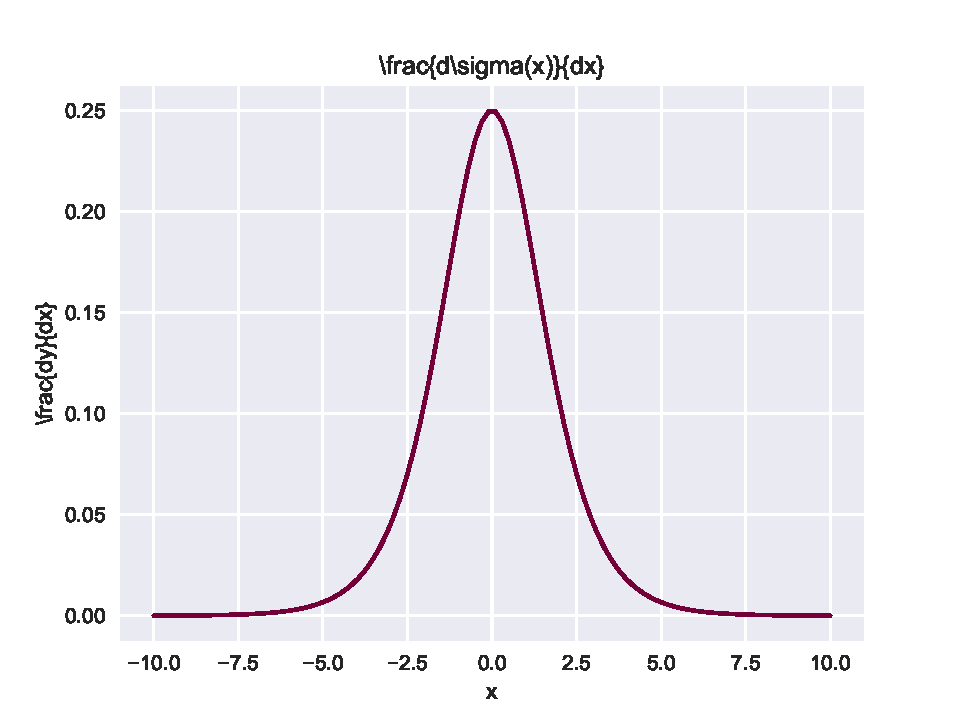
\includegraphics[width=0.45\linewidth,angle=0]{sigmoid_derivative.pdf}
% \caption{sigmoid derivative}
}
\end{centering}
\caption{sigmoid activation function and its derivative}

\end{figure}

\subsection{tanh}
Tanh is good. It's a nonlinear function, like sigmoid, but for zero input it returns zero output. The mean of this function (given uniform x) is zero, so it handles centred data very well ( zero input gives zero output).
The tanh function (sinh/cosh) and its derivative are given by
\begin{eqnarray*}
\mathrm{tanh}(x) & = &\frac{e^x\,-\, e^{-x}}{e^x\,+\, e^{-x}} \\
\frac{d\sigma(x)}{dx} & = & 1 - \mathrm{tanh}^2(x) 
\end{eqnarray*}

these are plotted below
\begin{figure}[tb]
\begin{centering}
\subfigure{
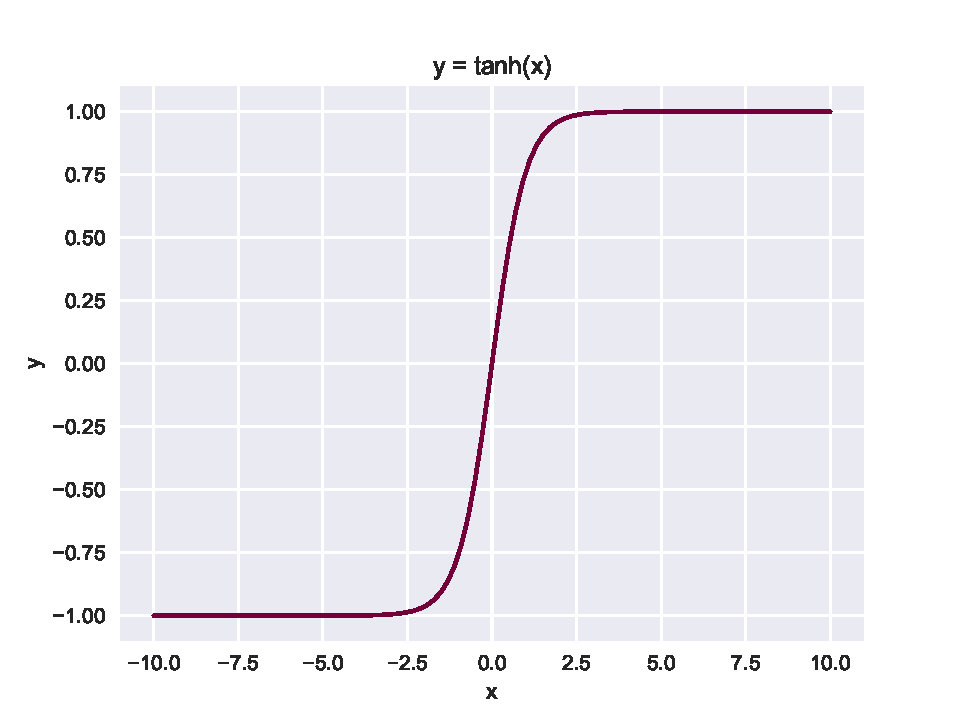
\includegraphics[width=0.45\linewidth,angle=0]{tanh.pdf}
}
\subfigure{
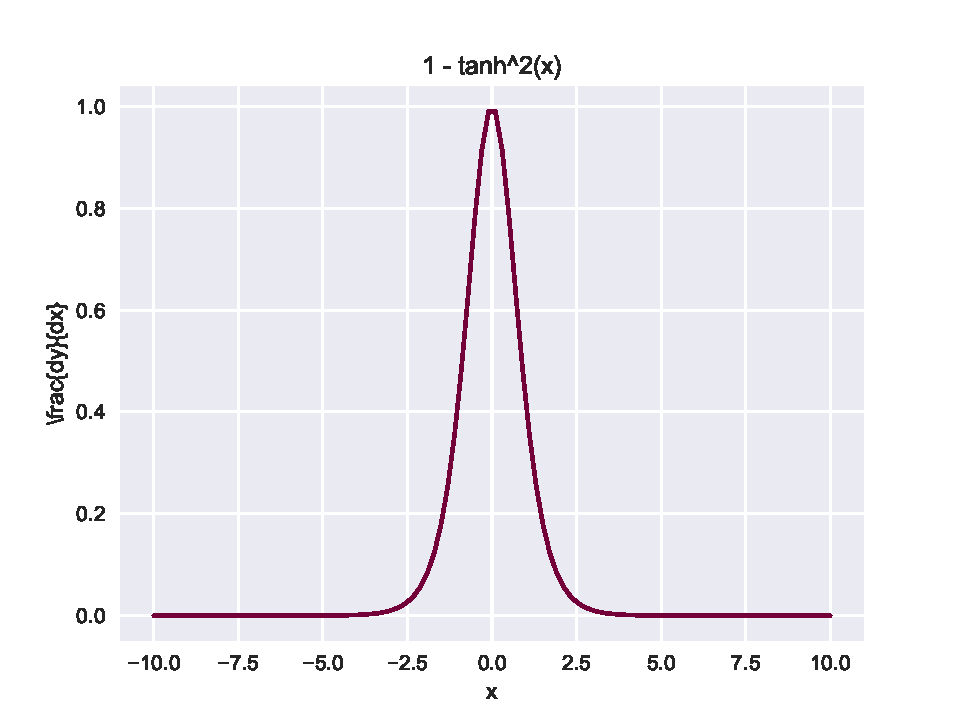
\includegraphics[width=0.45\linewidth,angle=0]{tanh_derivative.pdf}
% \caption{tanh derivative}
}
\end{centering}
\caption{tanh activation function and its derivative}
\end{figure}

\subsection{ReLu}
rectified linear unit. Max(0,x). This is a very popular activation, as it tends to give good results. Should in general be the first choice for an activation function (rather than sigmoid/tanh, though there may be cases where these perform better).
\begin{figure}[tb]
\begin{centering}
\subfigure{
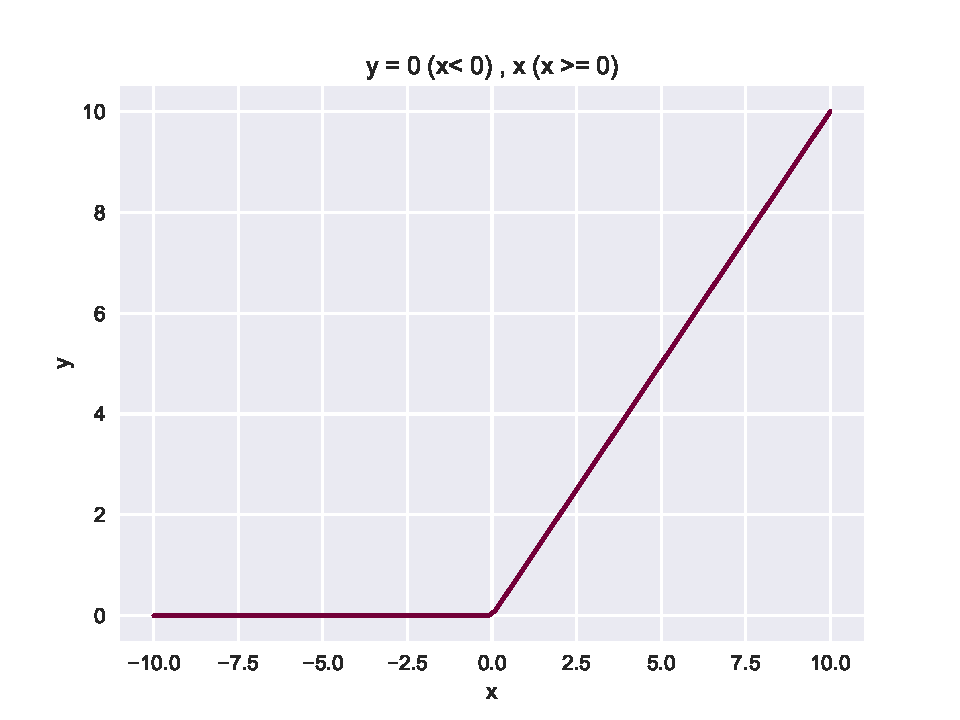
\includegraphics[width=0.45\linewidth,angle=0]{ReLu.pdf}
% \caption{tanh activation function}
}
\subfigure{
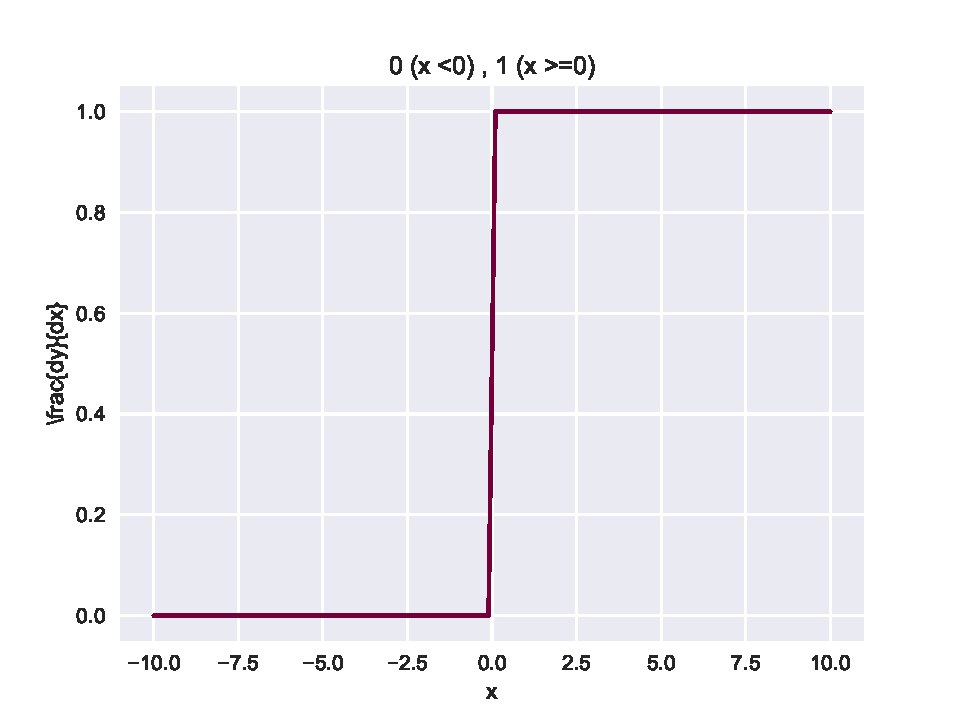
\includegraphics[width=0.45\linewidth,angle=0]{ReLu_derivative.pdf}
% \caption{tanh derivative}
}
\end{centering}
\caption{ReLu activation function and its derivative}
\end{figure}

\subsection{leaky ReLu}
Gradient saturation and such. If a Relu Network ever gets to a state where the inputs are large and negative, all the gradients will vanish, and the network will stop updating, it gets stuck. Leaky Relu has a very small (1\%) output for negative x, so the gradient never fully vanishes. It's a little more robust
\begin{figure}[tb]
\begin{centering}
\subfigure{
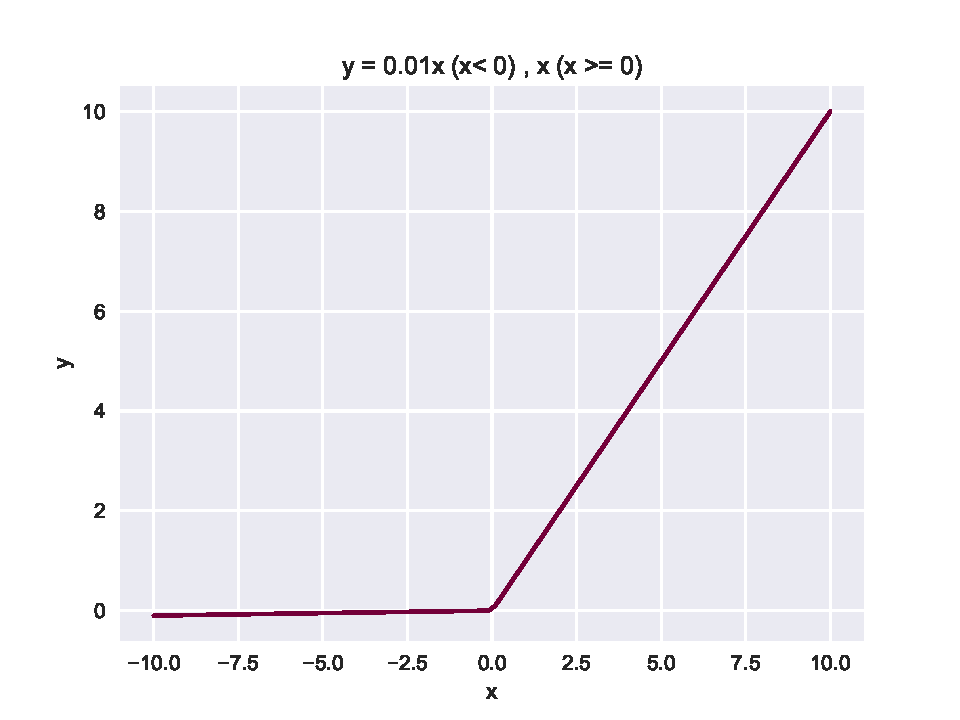
\includegraphics[width=0.45\linewidth,angle=0]{leaky_ReLu.pdf}
% \caption{tanh activation function}
}
\subfigure{
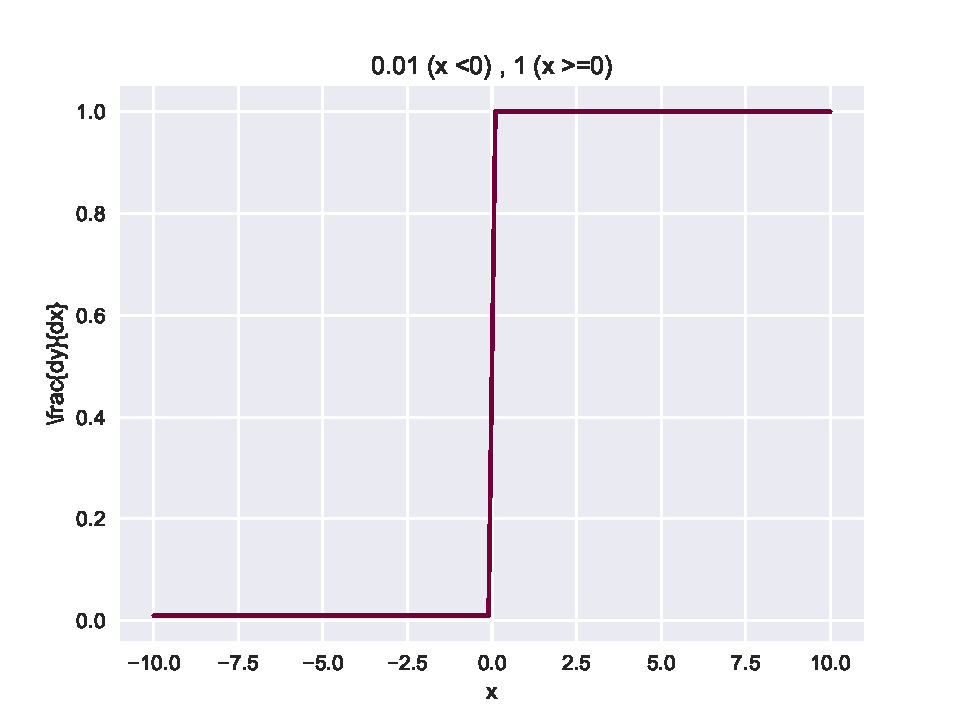
\includegraphics[width=0.45\linewidth,angle=0]{leaky_ReLu_derivative.pdf}
% \caption{tanh derivative}
}
\end{centering}
\caption{Leaky Relu activation function and its derivative}

\end{figure}

\section{regularisation/tuning}
\subsection{dropout}
inverted dropout


\end{document}

